\subsection{Software Privilege Levels}
\label{sec:rings}

In an Infrastructure-as-a-Service (IaaS) cloud environment, such as Amazon EC2,
commodity CPUs run software at four different privilege levels. A solid
understanding of Intel architecture's privilege stack is a vital piece of
context for analyzing SGX.

Figure~\ref{fig:cpu_rings} shows the privilege levels in the Intel
architecture. Software running at each level is strictly more powerful than
software running at less privileged levels. It follows that software running at
a level can access the code and data at less privileged levels, and compromise
the software running at these levels. Thus, software at each level must trust
all the software running at more privileged levels.

\begin{figure}[hbtp]
  \centering
  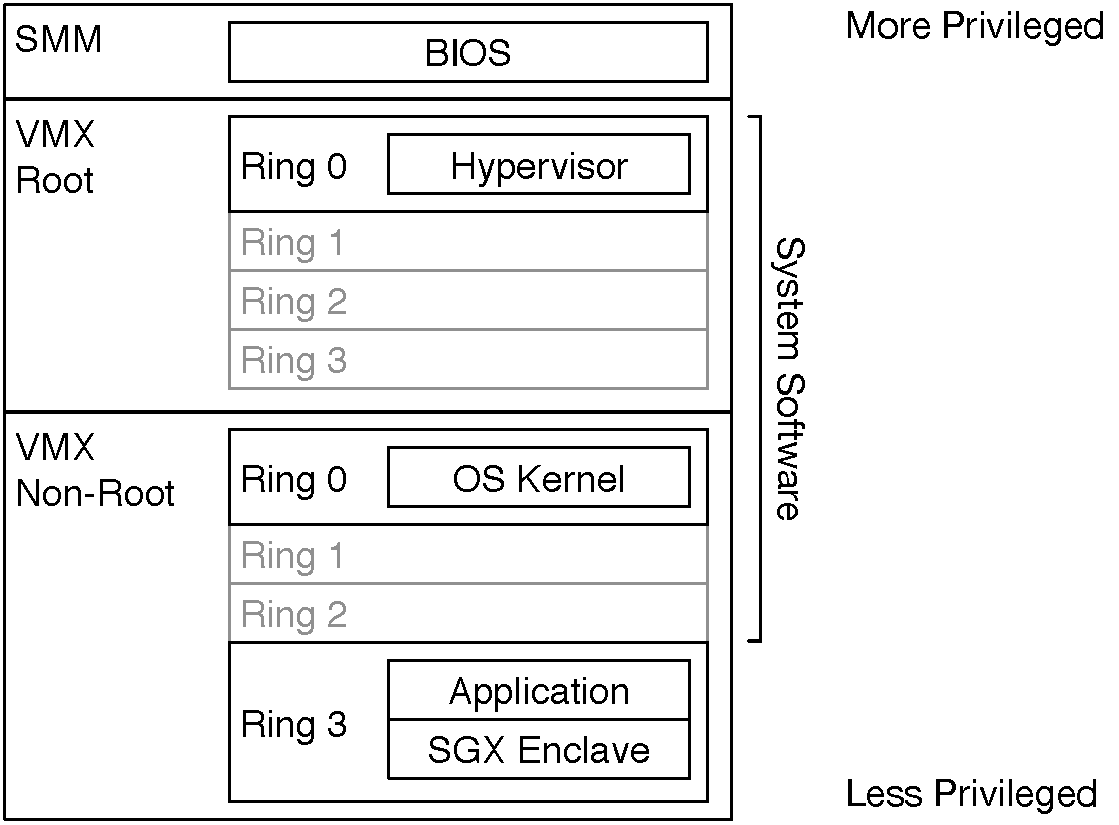
\includegraphics[width=85mm]{figures/cpu_rings.pdf}
  \caption{
    The privilege levels in the x86 architecture, and the software that
    typically runs at each security level.
  }
  \label{fig:cpu_rings}
\end{figure}

% System Management Mode: SDM S 34

\textit{System Management Mode} (SMM) is intended for use by the motherboard
manufacturers to implement features such as fan control and deep sleep, and/or
to emulate missing hardware. Therefore, the bootstrapping software
(\S~\ref{sec:booting}) in the computer's firmware is expected to load all the
SMM code inside a special continuous subset of DRAM, called the \textit{System
Management RAM} (SMRAM), and is expected to set up hardware protections
preventing less privileged software from accessing the SMRAM.

IaaS cloud providers allow their customers to run their operating system of
choice in a virtualized environment. Hardware
virtualization~\cite{uhlig2005vmx}, called \textit{Virtual Machine Extensions}
(VMX) by Intel, adds support for a \textit{hypervisor}, also called a
\textit{Virtual Machine Monitor} (VMM) in the Intel documentation. The
hypervisor runs at a higher privilege level (VMX root mode) than the operating
system, and is responsible for allocating hardware resources across multiple
operating systems that share the same physical machine. The hypervisor uses the
CPU's hardware virtualization features to make each operating system believe it
is running in its own computer, called a \textit{virtual machine} (VM).
Hypervisor code generally runs at ring 0 in VMX root mode.

Hypervisors that run in VMX root mode and take advantage of hardware
virtualization generally have better peformance and a smaller codebase than
hypervsiors based on binary translation \cite{rosenblum2005virtualization}.

The systems research literature recommends breaking up an operating system into
a small \textit{kernel}, which runs at a high privilege level, known as the
\textit{kernel mode} or \textit{supervisor mode} and, in the Intel
architecture, as \textit{ring 0}. The kernel allocates the computer's resources
to the other system components, such as device drivers and services, which run
at lower privilege levels. However, for performance reasons\footnote{Switching
between rings is much slower than a normal procedure call.}, mainstream
operating systems have large amounts of code running at ring 0. Their
\textit{monolithic kernels} include device drivers, filesystem code, networking
stacks, and video rendering functionality.

Application code, such as a Web server or a game client, runs at the lowest
privilege level, referred to as \textit{user mode} (\textit{ring 3} in the
Intel architecture). In IaaS cloud environments, the virtual machine images
provided by customers run in VMX non-root mode, so the kernel runs in VMX
non-root ring 0, and the application code runs in VMX non-root ring 3.
